% ycb1-fig-vertebral-column. Labels from notes block ycb1-hl-human-body-introduction,
% "Vertebral column" bullet (checked: regions 7, 12, 5, fused sacrum and coccyx).
\documentclass[border=6pt]{standalone}
% Shared preamble for the YCB1 line diagrams (standalone TikZ, XeTeX). Black and white only; labels come from
% the checked notes block named in each diagram file. Build: make_figures.bat in this folder.
\usepackage{fontspec}
\setmainfont{Segoe UI}
\usepackage{tikz}
\usetikzlibrary{arrows.meta,positioning,shapes.geometric,calc,decorations.pathreplacing}
\hyphenpenalty=10000 \exhyphenpenalty=10000 % no hyphenated labels
\tikzset{
  box/.style={draw, rounded corners=2pt, align=center, inner sep=4pt, font=\small, minimum height=1.6em},
  head/.style={box, font=\small\bfseries},
  note/.style={align=center, font=\footnotesize},
  link/.style={-{Stealth[length=2mm]}, thin},
}

\begin{document}
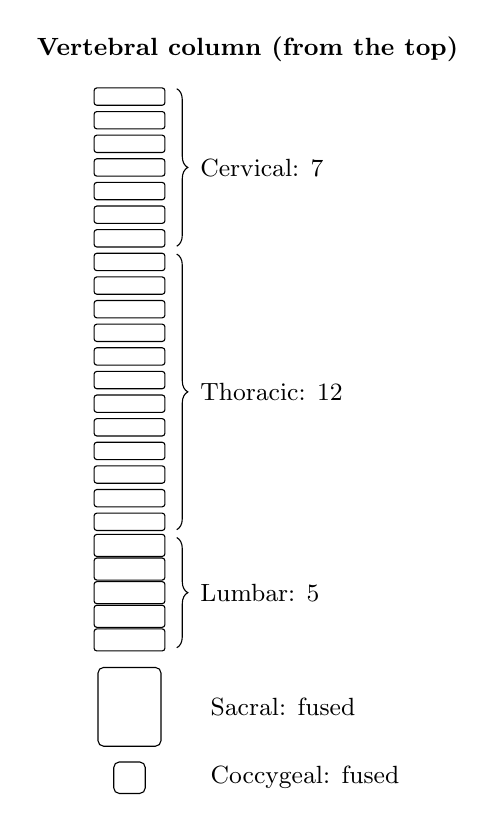
\begin{tikzpicture}[v/.style={draw, rounded corners=1pt, minimum width=9mm, minimum height=2.2mm, inner sep=0pt}]
\node[font=\small\bfseries] at (1.5,0.6) {Vertebral column (from the top)};
% one small block per vertebra; fused regions as one longer block
\foreach \i in {0,...,6}  \node[v] at (0,-0.3*\i) {};
\foreach \i in {7,...,18} \node[v] at (0,-0.3*\i) {};
\foreach \i in {19,...,23} \node[v, minimum height=2.8mm] at (0,-0.3*\i) {};
\node[draw, rounded corners=2pt, minimum width=8mm, minimum height=10mm] (sac) at (0,-7.75) {};
\node[draw, rounded corners=2pt, minimum width=4mm, minimum height=4mm] (coc) at (0,-8.65) {};
% region labels with braces on the right
\foreach \a/\b/\t in {0/6/{Cervical: 7}, 7/18/{Thoracic: 12}, 19/23/{Lumbar: 5}}
  \draw[decorate, decoration={brace, amplitude=4pt}] (0.6,{-0.3*\a+0.1}) -- (0.6,{-0.3*\b-0.1})
     node[midway, right=5pt, font=\small] {\t};
\node[right=5mm of sac, font=\small] {Sacral: fused};
\node[right=7mm of coc, font=\small] {Coccygeal: fused};
\end{tikzpicture}
\end{document}
